\chapter{Model Railroad Information Manager}
\section{Introduction}
\gls{rails} is a software model and implementation of an automated system to assist the model railroader achieve realism in the operation of a model railroad.
The \gls{rails} system design describes the system's architecture, components, and interfaces and can be found at \href{https://github.com/djbristow/RAILS/blob/master/Documentation/rails-system.pdf}{RAILS System Design and implementation}.
There are four user interface \glspl{spa} that provide different aspects of \gls{rails} they are:
\begin{itemize}
  \item \gls{rsrm} provides a user with a web application to show, when an RFID tag is read, the road name and number of the rolling stock associated with that tag.
  \item \gls{mrim} the focus of this manual, allows the user to create, update and delete model railroad assets, such as:
    \begin{itemize}
		\item manage lists of items found in model railroads:
        \begin{itemize}
 		    \item Rolling Stock
 		    \item DCC decoders
 		    \item AAR Codes
 		    \item Images
 		    \item Companies
 		    \item Structures
	    \end{itemize}
		\item creates PDF reports; and
        \begin{itemize}
 		    \item AAR Codes
 		    \item Companies
 		    \item Images
 		    \item RFID
 		    \item Rolling Stock sortable by Road Name and Road Number or AAR Code or Status
	    \end{itemize}
		\item exports and imports inventories in CSV files.
	\end{itemize}
  \item \gls{mppm} allows the user to enter information about their projects and purchases; and
  \item \gls{mrlm} allows the user to enter information about their layout and control elements of it.
\end{itemize}
\section{Components}
The implementation of \gls{mrim} consists of the following microservices components:
\begin{itemize}
    \item \gls{mrfm} provides the user the ability to upload image files;
    \item images is a repository for the images of rollingstock and structures;
    \item \gls{rids} provides \gls{rest} access to railroad inventory collections including \gls{rs};
    \item MongoDB a NoSQL database program that stores data records as documents which are gathered in collections. A database stores one or more collections of documents;
    \item \gls{mr} Data is the document repository, used by MongoDB, to store complete collections of items such as \gls{rs}, industries (producers and consumers), track elements, 
turnouts, projects, purchases, etc. in support of \gls{rails}; and
    \item \gls{mrim} is the \gls{spa}.
\end{itemize}
\begin{figure}[H]
	\centering
		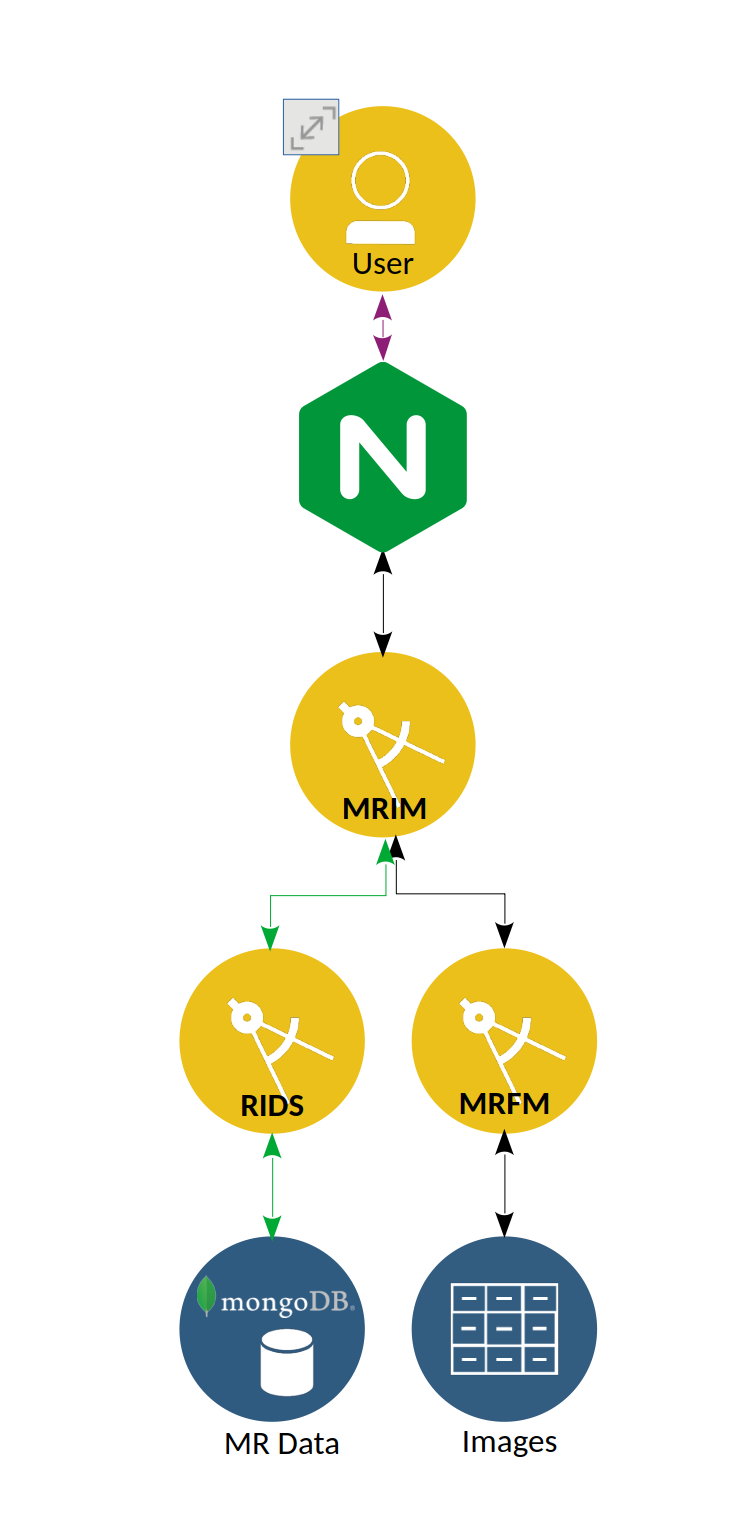
\includegraphics[scale=0.2]{./images/mrim-design.png}
	\caption{Microservices Components}
	\label{fig:rsms-ms-components}
\end{figure}
\section{System Components}
Three system components that make up this subsystem:
\begin{itemize}
    \item Network is a \gls{tcpip} communication medium that connects the client (one or more) to the host running the \gls{mrim} docker containers;
    \item Server is a computer that runs \gls{mrim} microservices components; and
    \item Client\footnote{A web browser may be used on the Server and client machine is omitted} is a computer that runs a web browser to display the \gls{mrim} \gls{spa}.
\end{itemize}

\begin{figure}[H]
	\centering
		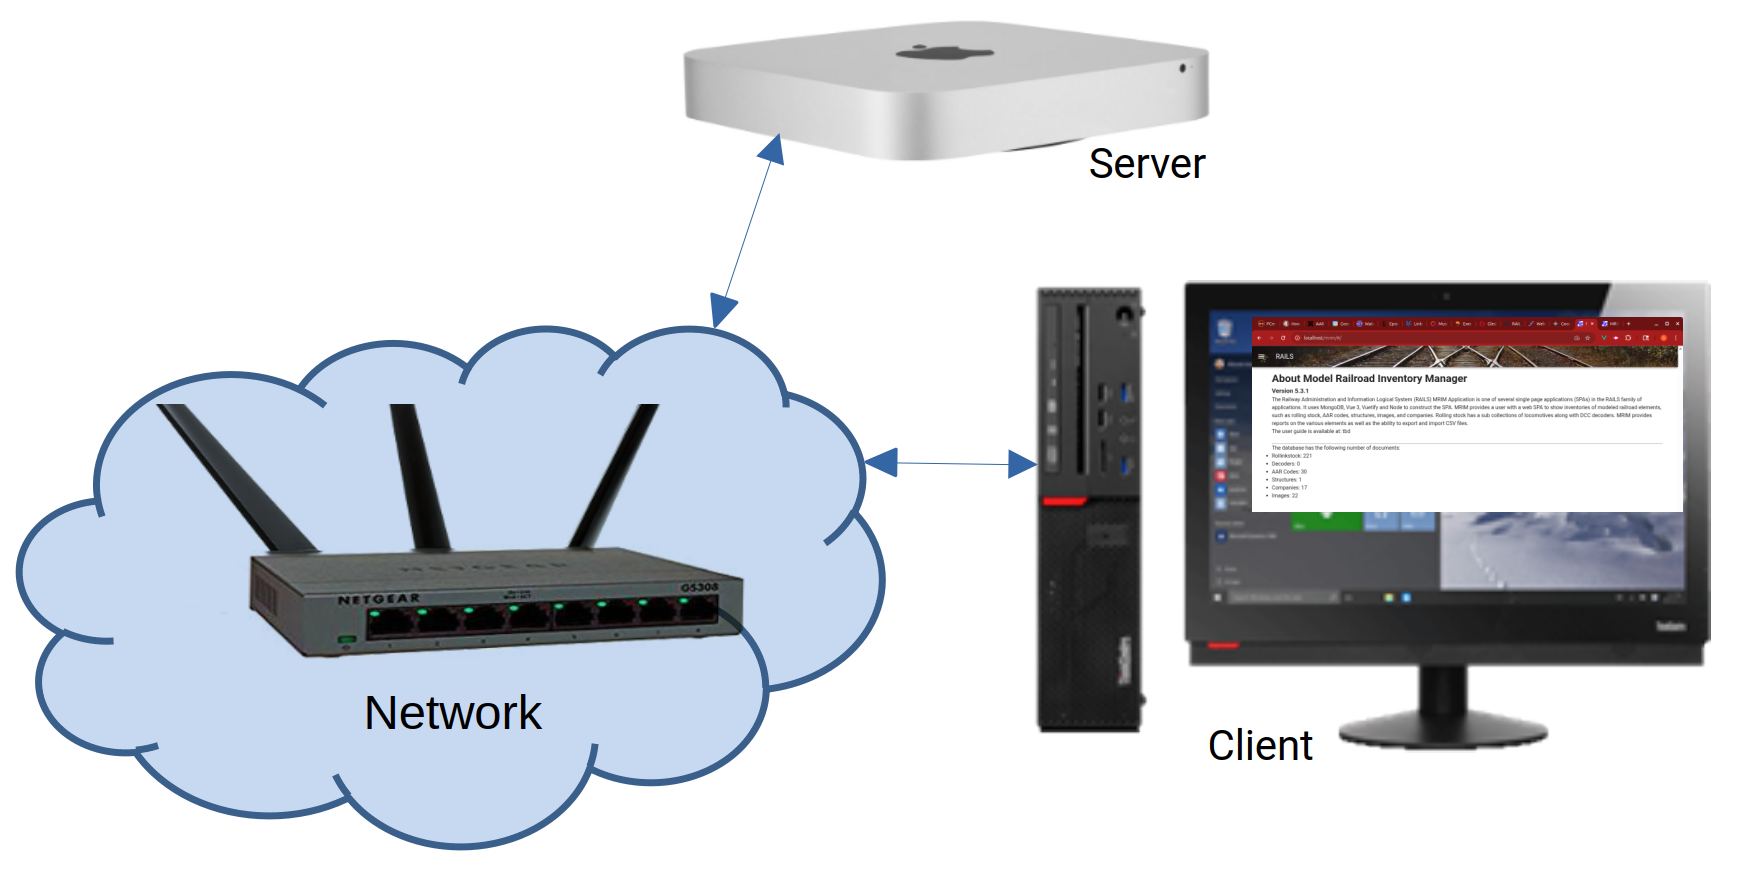
\includegraphics[scale=0.25]{./images/mrim-system.png}
	\caption{System Components}
	\label{fig:mrim-system-components}
\end{figure}
